\documentclass[thesis=B,czech]{FITthesis}[2012/06/26]

\usepackage[utf8]{inputenc} % LaTeX source encoded as UTF-8

\usepackage{graphicx} %graphics files inclusion
% \usepackage{amsmath} %advanced maths
% \usepackage{amssymb} %additional math symbols
\usepackage[figuresleft]{rotating}
\usepackage[flushleft]{threeparttable} % for footnote in tabular

\usepackage{dirtree} %directory tree visualisation

\usepackage{enumitem}
\setlist[enumerate]{label*=\arabic*.}

% % list of acronyms
% \usepackage[acronym,nonumberlist,toc,numberedsection=autolabel]{glossaries}
% \iflanguage{czech}{\renewcommand*{\acronymname}{Seznam pou{\v z}it{\' y}ch zkratek}}{}
% \makeglossaries

\newcommand{\tg}{\mathop{\mathrm{tg}}} %cesky tangens
\newcommand{\cotg}{\mathop{\mathrm{cotg}}} %cesky cotangens

% Macros to use as research features criteria. 
% The text is used repeatedly, so in case of its change I want the change
% to happen everywhere.
\newcommand{\crita}{Nevyžaduje vlastní infrastrukturu, rychlé zprovoznení}
\newcommand{\critb}{Použitelnost}
\newcommand{\critc}{Absence nepotrebné funkcionality}
\newcommand{\critd}{Použití zdarma}
\newcommand{\crite}{Funkce}
\newcommand{\critf}{REST API}
\newcommand{\critg}{Open-source}

\department{Katedra Softwarového Inženýrství}
\title{Systém správy úkolů pro jednotlivce a malé týmy}
\authorGN{Martin} %(křestní) jméno (jména) autora
\authorFN{Melka} %příjmení autora
\authorWithDegrees{Martin Melka} %jméno autora včetně současných akademických titulů
\supervisor{Ing. Josef Pavlíček, Ph.D.}
\acknowledgements{Doplňte, máte-li komu a za co děkovat. V~opačném případě úplně odstraňte tento příkaz.}

\abstractCS{Tato bakalářská práce se zabývá srovnáním existujících aplikací a tvorbou nové aplikace pro správu úkolů. Uživateli této aplikace budou jednotlivci a menší pracovní skupiny, a přidělovat a sledovat průběh práce na společných úkolech. Aplikace umožní lidem sdružovat se do skupin, spolupracovat na sdílených úkolech a zaznamenávat odvedenou práci. Součástí této práce je definice požadavků na aplikaci, srovnání navrhovaného řešení s existujícími aplikacemi, dále návrh, implementace, testování a nasazení aplikace. Výsledkem práce bude aplikační backend, vystavující funkcionalitu skrze REST rozhraní.}

\abstractEN{The aim of this thesis is to compare available software applications for task management and to subsequently create an original one. The users of this application will be individuals and small-scale workgroups, who need to assign responsibilities for and track the progress of shared tasks. The application will allow users to form groups, work together on shared tasks and report the work done on them. This thesis consists of a definition of application requirements, comparison of current task management solutions and design, implementation, testing and deployment of the proposed application. The outcome of this thesis will be an application backend, which exposes its functionality through a REST interface.}
\placeForDeclarationOfAuthenticity{V~Praze}
\declarationOfAuthenticityOption{4} %volba Prohlášení (číslo 1-6)
\keywordsCS{Správa úkolů, produktivita, organizace týmů, backend, REST, Java Spring Framework}
\keywordsEN{Task management, productivity, team organization, backend, REST, Java Spring Framework}

\begin{document}

% \newacronym{CVUT}{{\v C}VUT}{{\v C}esk{\' e} vysok{\' e} u{\v c}en{\' i} technick{\' e} v Praze}
% \newacronym{FIT}{FIT}{Fakulta informa{\v c}n{\' i}ch technologi{\' i}}

\begin{introduction}
	Výpočetní technika umožnila rozvoj rychlejší a efektivnější komunikace, práce a vůbec způsobu života. Je běžné mít svůj kalendář on-line a sdílet ho s ostatními, případně používat některý nástroj s funkcí úkolníčku. Zejména ve velkých firmách, kde existuje silná potřeba koordinovat úsilí mnoha lidí, tak vznikla poptávka po nástrojích pro správu úkolů, které by jim umožnily efektivnější rozdělování zodpovědností a práce. Řešení, které na tento popud vznikly, slouží právě potřebám velkých firem. Potřeby menších skupin a jednotlivců jsou ale jiné. Pro ně jsou tyto nástroje příliš komplexní, těžkopádné a nedostatečně intuitivní.

	Tato práce se zabývá přehledem existujících řešení pro správu úkolů malých i velkých skupin a tvorbou backendu nové aplikace. Aplikace bude zaměřena na potřeby menších týmů a jednotlivců a bude umožňovat uživatelům vytvářet úkoly, sdílet je s ostatními uživateli, sdružovat se do skupin a zaznamenávat průběh práce na úkolech. 
	
	V první části porovnám současná řešení pro správu úkolů z pohledu malých týmů a jednotlivců. 
	
	Ve druhé části se zabývám analýzou problému. Definuji požadavky na aplikaci ve formě uživatelských příběhů a podrobím je analýze.
	
	Ve třetí části vypracuji návrh řešení aplikace. Zde vybírám technologii pro implementaci a popisuji architekturu aplikace, návrhový model tříd a databázový model.
	
	Ve čtvrté části popisuji implementaci aplikace.
	
	V páté části se věnuji testování aplikace za účelem zjištění její správné funkčnosti. Popíšu zde použité technologie a způsob testování.
	
	V poslední, šesté části, vysvětlím, jak výslednou aplikaci nasadit a spustit.
\end{introduction}

%%%%%%%%%%%%%%%%%%%%%%%%%%%%%%%%%%%%%%%%%%%%%%%%%%%%%%%%%%%%%%%%%%%%%%%%%%%%%%%%%%%%%%%%%%%%%%%%%%%%%%%%%
%%%%%%%%%%%%%%%%%%%%%%%%%%%%%%%%%%%%%%%%%%%%%%%%%%%%%%%%%%%%%%%%%%%%%%%%%%%%%%%%%%%%%%%%%%%%%%%%%%%%%%%%%
\chapter{Slovník pojmů}
	\begin{description}
		\item[Deadline] je časová lhůta, do které je nutné dokončit nějakou práci. Jeho synonyma jsou uzávěrka a konečný termín.
		
		\item[Assignee] je člověk přidělený k určitému úkolu, je zodpovědný za práci na něm.
		\item[Open source software] je softwarové dílo, k němuž jsou veřejně dostupné jeho zdrojové kódy.
		\item[Closed source software] je softwarové dílo, jehož zdrojové kódy nejsou veřejně dostupné.
		\item[Gamifikace] je uplatňování technik z herního designu a herních principů do neherních oblastí. Slouží například k motivaci formou získávání bodů za určité činnosti a zobrazováním grafů jejich vývoje.
		\item[Backend] je část webové aplikace, která nekomunikuje přímo s uživatelem. V kontextu této práce zprostředkovává aplikační logiku a s okolím komunikuje skrze definované rozhraní.
		\item[Manhour] je jednotka práce. Jeden člověk odpracuje za hodinu jeden \textit{manhour}. Vypočte se jako: $manhours = lidi \times hodiny$.
		\item[Embedded] znamená vestavěný, zabudovaný. 
	\end{description}
\chapter{Současný stav}
	\label{chapter:current-state}

	Způsobů, jak řešit správu úkolů, existuje spoustu a liší se podle toho, kdo je má využívat. V této části práce představím několik zástupců pro každou ze tří kategorií. Těmi jsou:
	\begin{enumerate}
	  \item Řešení pro větší firmy s množstvím pracovníků
	  \item Řešení pro střední a menší týmy, jednotky až desítky pracovníků
	  \item Řešení pro jednotlivce
	\end{enumerate}

	Zástupce vybírám podle osobních zkušenosti a podle výsledků získaných z vyhledávače \texttt{Google}, na základě jejich pořadí a popularity mezi uživateli. U uvedených zástupců uvedu krátký popis a jejich použitelnost cílovou skupinou této práce, tj. menšími týmy a jednotlivci.

	Pracuji s tím, že pro cílovou skupinu této práce jsou důležitá následující kritéria:
	\begin{enumerate}
		\item \textbf{\crita} -- Uživatelé nechtějí spravovat vlastní hardware, kde by jim aplikace běžela. Začít používat aplikaci má být otázka maximálně několika málo minut.
		\item \textbf{\critb} -- Kritérium jsem hodnotil subjektivně, podle mého názoru na pět kvalitativních částí použitelnosti\cite{usability}. Uživatel by se neměl ztratit ve funkcích aplikace a měl by být schopen rychle pochopit, jak s aplikací pracovat. 
		\item \textbf{\critc} -- 	Aplikace by měla obsahovat jen základní funkce, které uživatel využije. Větší množství funkcí, které uživatele nezajímají, ztěžují orientaci v aplikaci, což souvisí s předchozím bodem.
		\item \textbf{\critd} -- Aplikace by měla být použitelná zdarma. V případě, že se jedná o \textit{freemium} model, měla by její neplacená část stačit k běžnému používání a neomezovat výrazně uživatele.
		\item \textbf{\critf} -- Aplikace by měla nabízet rozhraní REST API pro možnost vlastní integrace na její funkce.
		\item \textbf{\critg} -- Aplikace by měla mít veřejně dostupné zdrojové kódy.
	\end{enumerate}
	Uvedený přehled není vyčerpávající, věnuji se jen některým z těch nejznámějších řešení. 

	\section{Řešení pro firmy}
		\label{sec:solutions-companies}
		Řešení této kategorie se zaměřují na větší počet uživatelů a mimo základní správy úkolů nabízí často další funkce pro řízení projektů a integraci s dalšími systémy. Používají se zejména v oblasti vývoje software, ale dají se využít i v jiných oblastech.
		
		\subsection{JIRA}
			JIRA \cite{jira} je software, který nabízí bug tracking, issue tracking a funkce pro správu projektů. Je možné ho používat jak na vlastní HW infrastruktuře, tak on-line. V prvním případě je použití zdarma za určitých podmínek\footnote{Zdarma pro veřejně dostupný open-source software projekt\cite{jira-lic-opensource} a pro neziskové, nevládní, neakademické, nekomerční a sekulární instituce, které by si jinak nemohly software dovolit. \cite{jira-lic-nonprofit}}, v druhém případě je použití placené. 
			
			Nabízí širokou funkcionalitu a např. možnost upravovat podle potřeb životní cyklus úkolů. To ho činí využitelným i mimo vývoj software. Množství nabízených funkcí jde ale nad potřeby cílové skupiny této práce a technicky méně zdatné uživatele může mást. Na úkolech lze pracovat ve více lidech, ale přiřazen může být v jednu chvíli jen jednomu uživateli (\textit{assignee}). Úkolům lze také přiřadit \textit{deadline}.
			
			JIRA nabízí REST API a je closed source.
			
		\subsection{Bugzilla}
			Bugzilla \cite{bugzilla} je bug tracking nástroj, který je zaměřen hlavně na vývoj software. Je podobný nástroji JIRA, nicméně nenabízí takovou flexibilitu a i když by mohl být s dobře nastavenou politikou použitý pro správu úkolů u jiných než softwarových projektů, nebylo by použití intuitivní. Samotná správa a práce s úkoly funguje stejně jako u nástroje JIRA.
			
			Bugzilla je open source, licencovaná pod MPL, a lze ji využít zdarma i pro komerční účely. Je nutné ji ale provozovat na vlastním hardware. Existují hosting služby, které jsou ale neoficiální a placené. Bugzilla nabízí REST API.
			
		\subsection{Redmine}		
			Redmine \cite{redmine} je issue tracking nástroj, který nabízí více flexibility než Bugzilla a obsahuje i některé nástroje pro řízení projektů. Tyto nástroje mohou být přínosné pro větší projekty, které mají danou strukturu, ale nepočítám s tím, že by cílovou skupinu této práce zajímaly. Funkcionalita, která se týká správy úkolů, je srovnatelná s předchozími dvěma nástroji.
			
			Použití je zdarma, ale je nutné nainstalovat na vlastním hardware. Stejně jako v případě Bugzilly není Redmine oficiálně použitelný on-line, soukromé hostingy jsou placené. Projekt je vyvíjen jako open source a nabízí REST API.

	\section{Řešení pro střední a menší týmy}
		\label{sec:solutions-teams}
		Nástroje v této kategorii se snaží cílit na týmy, spíše než celé firmy, a práce s nimi není tak formální. Používat je lze on-line, není nutné vlastní instalace. Oproti řešením v bodu \ref{sec:solutions-companies} obsahují tyto méně funkcí, chybí hlavně různé manažerské nástroje a integrace s dalšími systémy.
	
		\subsection{Trello}
			Trello \cite{trello} je on-line aplikace, která vznikla v roce 2011. Způsob správy úkolů staví na konceptu \textit{kanban}\cite{kanban}. Umožňuje vytvářet nástěnky (boards), které reprezentují projekty. K nástěnkám lze přizvat další uživatele a pracovat na nich společně. Na nástěnkách se dají vytvářet seznamy (lists) a v nich karty (cards), které představují nejmenší jednotku práce - úkol. Ten má svou prioritu, \textit{deadline} a zodpovědné uživatele. Těch může být libovolný počet.
			
			Funkčně bohatý nástroj, s jednoduchým ovládáním i pro netechnické uživatele. Na profilu uživatele lze zobrazit všechny přiřazené karty a ty seřadit podle nástěnky, kam patří, nebo podle \textit{deadlinu}. 
			
			Trello je možné používat zdarma s libovolným počtem spolupracovníků. Placené varianty přináší určité výhody\cite{trello-pricing}, ale menší týmy se moho obejít bez nich. Existuje i REST API\cite{trello-api}, aplikace je \textit{closed source}.
		
			
		\subsection{Trackie}
			Trackie \cite{trackie} je on-line aplikace, která je určena pro správu úkolů na společných projektech. Ty lze zakládat a zvát do nich uživatele, v rámci projektů pak tvořit úkoly. Úkol může být někomu přiřazen, ale vždy jen jednomu uživateli. Funkčností i vzhledem jednoduché na použití, ale některé funkce oproti předchozím nástrojům chybí. Úkolům například nelze nastavit \textit{deadline}. Zobrazit je možné jen úkoly každého projektu zvlášť, nelze zobrazit přehled všech úkolů uživatele. 
			
			Aplikace nabízí 30denní zkušební dobu, po její uplynutí je placená. Nenabízí REST API a je closed source.
			
		\subsection{FogBugz}
			FogBugz \cite{fogbugz} je nástroj řízení projektů, který kromě issue trackingu nabízí i možnost agilního plánování\cite{agile-planning}, správu podpory a zpětné vazby zákazníků, vytváření dokumentu ve stylu Wiki a další. Nabídkou funkcí je nejbohatší z trojice nástrojů v této kategorii, i přesto se v aplikaci uživatel neztratí. 
			
			Uživatelé spolu mohou pracovat na úkolech (cases), které se dělí do projektů (projects). Na úkolu lze evidovat informace potřebné pro využití agilní metodiky plánování, včetně \textit{story points}. Úkolu je možné určit zodpovědného uživatele, odhad pracnosti a deadline. Na úkolu je možné průběžně zaznamenávat odpracovanou práci a zobrazovat kolik času na něm zbývá.
			
			FogBugz nabízí 7denní zkušební dobu zdarma, poté je nutné za používání platit. Je možné ho používat jak on-line, tak na vlastním hardware. Nabízí REST API a je closed source.

	\section{Řešení pro jednotlivce}
		\label{sec:solutions-individuals}
		Poslední kategorií jsou nástroje pro správu úkolů jednotlivců. Některé z nich mohou umožňovat sdílení úkolů, takže by se daly zařadit i do kategorie \ref{sec:solutions-teams}, nicméně svým zaměřením cílí primárně na využití jako osobní úkolníček, proto jsou zařazeny zde. Také jsem do této kategorie zařadil nástroje, které nejsou primárně určeny pro správu úkolů, ale někteří je k tomuto účelu využívají, například kalendář nebo poznámky.
		
		\subsection{Todoist}
			Todoist \cite{todoist} je on-line aplikace pro organizaci úkolů, která má uživatele motivovat k lepší produktivitě. Za splněné úkoly jsou přidělovány body (karma), jejichž historický vývoj je možné sledovat v grafu, lze nastavit denní a týdenní cíl a získávat další \uv{odměny} za jeho splnění. Úkoly lze rozdělit do projektů, nastavit jim \textit{deadline}, prioritu a opakování. Projekty je možné sdílet s dalšími uživateli a dají se zobrazit buď po projektech, ke kterým patří, nebo všechny na jednom místě -- ve schránce (inbox). 
			
			Vytvoření nového úkolu se může provést zadáním (anglického) textu, aplikace sama rozpozná klíčová slova a není tak nutné nastavovat vlastnosti úkolů ručně. Například heslo \textit{Go jogging at 1 PM every day} vytvoří úkol \textit{Go jogging}, který má \textit{deadline} ve 13 hodin a opakuje se každý den. 
			
			Placená verze nabízí větší množství otevřených projektů a úkolů, hledání v úkolech, notifikace a další.\cite{todoist-compare-premium} Todoist nabízí REST API\cite{todoist-api} a je closed source.
			
		\subsection{Toodledo}
			Toodledo \cite{toodledo} je on-line aplikace, která kromě úkolů umožňuje vytvářet si zvyky (habits). To jsou úkoly, které se opakují ve volitelné dny každý týden, jež mají uživatelům pomoci vypěstovat si a dodržovat dobré návyky. Po vykonání zvyku je možné označit ho za splněný a přidat k jeho splnění číslo nebo hodnocení. Mezi další možnosti patří poznámky (notes), seznamy (lists), nebo nástiny (outlines). 
			
			Úkoly lze třídit do složek, nastavit jim \textit{deadline} a prioritu. Spolupráce s dalšími uživateli vyžaduje placenou verzi aplikace a Webové rozhraní aplikace je oproti nástroji Todoist poměrně nepřehledné. Toodledo nabízí REST API\cite{toodledo-api} a je closed source.
			
		\subsection{Google Inbox Reminders}
			Inbox \cite{ginbox} je e-mailový klient od společnosti Google, který kromě práce s e-maily umožňuje vytváření jednoduchých úkolů (reminders). Ty lze kromě aplikace Inbox také zobrazit v kalendáři Google Calendar.\cite{gcal} Úkolům nelze nastavit \textit{deadline}, ale je možné je odložit (snooze) tak, aby se zobrazily později. Aktivní úkoly se zobrazují mezi příchozími e-maily.
			
			Úkoly nelze nijak třídit, ani u nich určovat prioritu. Jediná informace v úkolu je jeho popis. Pro základní potřeby dostačující, ale jinak funkčně chudý nástroj zatím nenabízí API\cite{ginbox-no-api} a je closed source.
			
			
			
		\subsection{Poznámky, kalendář}
			Tato sekce nepopisuje jeden konkrétní produkt, ale jejich skupinu. Uvádím je pro úplnost, jelikož je stále využívá velké množství lidí. Patří sem všechny nástroje pro psaní poznámek a vytváření událostí v kalendáři, a to jak elektronické, tak papírové. 
			
			Některé elektronické nástroje umožňují sdílení poznámek či kalendářů, takže se dají při dobře definovaných pravidlech použít i pro týmovou práci. Jejich použití je ale složitější s rostoucím počtem úkolů a projektů, protože neumožňují žádné filtrování, řazení úkolů ani přiřazování zodpovědností. Pro nenáročného uživatele, který si chce zapisovat nejdůležitější úkoly a sám se postará o to, že na nich nezapomene včas začít, může být toto řešení dostačující.
			
			Pro papírové \uv{nástroje} platí předchozí odstavec podobně, jen možnost spolupráce je ještě více omezena. A pokud celá skupina nemá společnou místnost pro práci, pak prakticky vyloučena. Navíc vzniká problém s archivací a uchováváním historie úkolů.
		
	
	\section{Shrnutí}
		Přehled kritérií stanovených na začátku kapitoly \ref{chapter:current-state} a jejich splnění uvedenými nástroji prezentuji v tabulce \ref{table:criteria} (příloha).
		
		Všechny nástroje umožňují vytvářet úkoly, ale v možnostech se liší. Nyní zvážím, které funkce jsou užitečné pro cílovou skupinu této práce a mají být obsaženy ve výsledné aplikaci. Při odkazování se k nástrojům nebo aplikacím v této sekci mám na mysli ty představené výše.
		
		Většina nástrojů umožňuje úkoly sdílet s jinými uživateli a společně s nimi pracovat na projektu. Možnost seskupit se do jednoho celku se spolupracovníky je užitečná, proto budou v aplikaci existovat pro uživatele pracovní skupiny.
		
		V aplikacích je u úkolu možné určit uživatele za něj odpovědné. Většinou lze přiřadit k úkolu v jednu chvíli jen jednoho uživatele, ale v nástroji Trello jich lze přiřadit libovolný počet. To může být pro některé typy úkolů užitečné. 
		
		Kromě \textit{deadlinu} a priority jako ve většině ostatních aplikací, lze ve FogBugz u úkolu nastavit i odhad pracnosti -- dobu, jakou by měla práce na úkolu trvat. Uživatel pracující na úkolu pak může průbězně zaznamenávat odpracovanou dobu a celá skupina tak vidí, v jaké fázi se úkol nachází. Toto chci zahrnout do výsledné aplikace a ještě rozšířit o další funkci. Na základě doby zbývající do \textit{deadlinu} a zbývající pracnosti na úkolu lze určit \uv{urgentnost}, tedy jakou má ještě uživatel rezervu, než \textit{deadline} zmešká. Tato informace o rezervě může uživatelům pomoct s rozhodováním, kterému úkolu se prioritně věnovat, aby jej ještě stihli.
		
		Například Todoist nabízí možnost vytvořený úkol opakovat v zadaném intervalu. Google Inbox kromě opakování umožňuje také úkol odložit na později, čímž uživateli zmizí z očí. V aplikaci chci vyjít z těchto funkcí a vytvořit funkci podobnou. Myšlenka je, že opakující se úkoly nebudou mít pevně daný \textit{deadline}. Uživatel se jim chce věnovat zhruba po nějakých intervalech, ale ne na den přesně. Při vytvoření úkol nebude důležitý, ale bude postupně nabývat na urgentnosti, až se důležitým stane. Poté uživatel úkol buď ukončí, nebo vynuluje a úkol znovu poroste.
		
		Backend část aplikace, jež bude výstupem této práce, bude zaměřením spadat na pomezí sekcí \ref{sec:solutions-teams} a \ref{sec:solutions-individuals}. Bude obsahovat vybrané funkce pro správu práce týmů i jednotlivců, které analyzuji v kapitole \ref{chapter:analysis}.

	
%%%%%%%%%%%%%%%%%%%%%%%%%%%%%%%%%%%%%%%%%%%%%%%%%%%%%%%%%%%%%%%%%%%%%%%%%%%%%%%%%%%%%%%%%%%%%%%%%%%%%%%%%
%%%%%%%%%%%%%%%%%%%%%%%%%%%%%%%%%%%%%%%%%%%%%%%%%%%%%%%%%%%%%%%%%%%%%%%%%%%%%%%%%%%%%%%%%%%%%%%%%%%%%%%%%	
\chapter{Analýza}
	\label{chapter:analysis}
	
	V této sekci se budu věnovat specifikování požadavků na aplikaci a jejich analýze. To mi poskytne konkrétní přehled o tom, co má výsledná aplikace umět a jaké entity v ní budou existovat.
	
	\section{Požadavky na aplikaci}
		Požadavky na aplikaci popíšu pomocí \textit{user stories} (uživatelské příběhy)\cite{user-stories}. Jedná se o jednoduchý způsob, jakým vyjádřit požadavek na aplikaci z pohledu jejího uživatele. Měl by být krátký a napsán v terminologii uživatele budoucí aplikace.
		
		Formální způsob zápisu user story se dá definovat \cite{user-stories-applied-book} například takto:
		\begin{center}
			Jako $\langle$role$\rangle$ chci $\langle$něco$\rangle$, abych dosáhl $\langle$něčeho$\rangle$.
		\end{center}
		Pomocí \textit{user stories} lze také testovat, zda aplikace obsahuje všechny požadované funkce. Pokud jsou všechny \textit{user stories} uspokojeny, pak je aplikace z hlediska funkčnosti hotova.
		
		\subsection{User stories}
		\label{sec:user-stories}
		\begin{enumerate}
			\item \textbf{Uživatel}
			\begin{enumerate}
				\item Jako uživatel chci mít svůj účet, abych mohl spravovat své úkoly a pracovní skupiny. Účet bude jednoznačně identifikován e-mailem uživatele a pro přihlášení bude potřeba heslo. Dále bude účet obsahovat jméno uživatele. Svůj účet budu moci zobrazit a upravit svoje jméno a heslo.
				
				\item Jako uživatel chci u úkolu mít vždy jednu ze dvou rolí -- pozorovatel a pracovník -- abych dal najevo, v jakém vztahu k úkolu jsem. Jako pozorovatel mám jen pasivní roli, úkol vidím ve svém seznamu. Jako pracovník se na úkolu aktivně podílím.
				
				\item Jako uživatel chci vytvářet úkoly soukromé nebo sdílené s ostatními uživateli a pracovními skupinami, abych nezapomněl na své nebo týmové úkoly, které je potřeba vypracovat. Úkol bude obsahovat následující informace:
				\begin{itemize}
					\item Název
					\item Popis
					\item Datum a čas začátku
					\item Pracnost (\textit{manhours})
					\item Priorita
					\item Typ
					\begin{itemize}
						\item S deadlinem -- úkol má daný \textit{deadline}, kdy má být splněn
						\item Rostoucí -- úkol nemá daný \textit{deadline}, ale jeho urgentnost postupně roste
					\end{itemize}
					\item Datum a čas \textit{deadlinu} (pro úkoly \uv{s deadlinem})
					\item Rychlost růstu urgentnosti (pro \uv{rostoucí} úkoly)
					\item Stav
					\begin{itemize}
						\item Otevřený
						\item Splněný
						\item Zavřený
					\end{itemize}
				\end{itemize}
				
				\item Jako pozorovatel nebo pracovník úkolu ho chci sdílet s dalšími uživateli 
				
				\item Jako pracovník úkolu ho chci modifikovat, abych mohl reagovat na případné změny. Změnit budu moct všechny údaje, kromě jeho typu.
				
				\item Jako uživatel chci znát \textit{urgentnost} úkolů, abych věděl, kterým úkolům se mám věnovat tak, abych stihl jejich deadline. Čím méně času zbývá na vypracování úkolu vzhledem k jeho pracnosti a deadlinu, tím více je urgentní.
				
				\item Jako uživatel chci zobrazit všechny úkoly, kterých jsem součástí -- moje osobní i sdílené se mnou nebo pracovní skupinou, již jsem členem -- abych měl přehled o tom, co je potřeba udělat. Zobrazení by mělo jít filtrovat a řadit podle následujících kritérií:
				\begin{itemize}
					\item Filtr
					\begin{itemize}
						\item Role (pozorovatel / pracovník)
						\item Typ
						\item Stav
						\item Vlastnictví (můj / sdílený se mnou)
						\item Priorita
					\end{itemize}
					\item Řazení
					\begin{itemize}
						\item Název
						\item Datum začátku úkolu
						\item Datum \textit{deadlinu}
						\item Rozpracovanost (kolik procentuelně odpracováno)
						\item Priorita
						\item Urgentnost
					\end{itemize}
				\end{itemize}
				
				\item Jako uživatel chci přijímat nebo zamítat příchozí návrhy na sdílení úkolů, abych se mohl rozhodnout, na kterých se chci podílet a na kterých ne.
				
				\item Jako pracovník úkolu na něm chci zaznamenávat odvedenou práci, abych měl já i mí spolupracovníci lepší představu o tom, kolik práce na něm zbývá.
				
				\item Jako pracovník úkolu ho prohlašovat úkol za splněný, uzavřený, nebo znovuotevřený, abych dal najevo, v jakém stavu se úkol nachází.
				
				\item Jako pracovník na \uv{rostoucím} úkolu chci vynulovat jeho urgentnost, aby poté, co jsem ho splnil, dočasně přestal být důležitý. Tuto funkci využiji při opakovaných úkolech.
				
				\item Jako uživatel chci zakládat pracovní skupiny a po založení se stát jejich adminem, abych se mohl sdružovat s dalšími uživateli a pracovat společně. Pracovní skupina obsahuje tyto informace:
				\begin{itemize}
					\item Název
					\item Popis
				\end{itemize}
				
				\item Jako uživatel chci vidět seznam skupin, jichž jsem členem, manažerem nebo adminem, a jejich detaily, abych rychle viděl, se kterými skupinami spolupracuji.
			\end{enumerate}
			
			
			\item \textbf{Manažer skupiny}
			\begin{enumerate}
				\item Jako manažer skupiny do ní chci zvát a odebírat z ní uživatele. Členům chci přiřazovat role pozorovatel nebo pracovník na úkolech, které jsou se skupinou sdíleny, abych tím mohl organizovat skupinu a rozdělovat zodpovědnost za práci mezi její členy. 
				
				\item Jako manažer skupiny chci vytvářet úkoly pro skupinu a přijímat nebo zamítat návrhy na sdílení úkolů s mou skupinou, abych mohl určovat, na čem má skupina pracovat.
				
				\item Jako manažer skupiny chci mít možnost odebrat ji z úkolu, který je s ní sdílen, aby úkoly, které již nejsou relevantní, nezůstávaly v seznamu úkolů skupiny.
			\end{enumerate}
			
			
			\item \textbf{Admin skupiny}
			\begin{enumerate}
				\item Jako admin skupiny chci mít možnost měnit její název a popis, abych je mohl udržovat aktuální.
				\item Jako admin skupiny chci jmenovat manažery skupiny, abych mohl pověřit další uživatele správou skupiny.
				\item Jako admin skupiny chci mít možnost přenechat svou roli jinému členovi skupiny, abych mohl skupinu opustit a ta pořád měla admina.
				\item Jako admin skupiny chci mít možnost skupinu zrušit.
			\end{enumerate}
		\end{enumerate}	
		
		\subsection{Nefunkční požadavky}
		\begin{enumerate}
			\item Aplikace bude dostupná přes REST API. Jedná se o pouze o backend, takže k dispozici nebude žádné grafické rozhraní.
			
			\item Aplikace nebude z důvodu bezpečnosti uchovávat hesla jako prostý text. Oveření bude provedeno vhodným způsobem, který znemožní únik hesel.
			
			\item Zdrojové kódy aplikace budou veřejně dostupné pod MIT licencí.
		\end{enumerate}
		
	\section{Model případů užití}
		\textit{User stories} ze sekce \ref{sec:user-stories} nyní budu specifikovat detailněji pomocí modelu případů užití (\textit{use case model}). \textit{User story} by měl obsahovat tolik informací, aby i technicky nezkušený uživatel dokázal pochopit, co má aplikace dělat. Oproti tomu případy užití popisují konkrétní interakce uživatele s aplikací, tedy chování, které má aplikace mít, aby splnila potřeby na ní kladené. \cite{user-stories-vs-use-cases}
		
		Případů užití typicky bude více než \textit{user stories}\cite{si-usecases}, protože \textit{user stories} jsou více obecné, a tak na pokrytí jednoho může být potřeba více interakcí s aplikací a tedy více případů užití.
		
		\subsection{Účastníci}
			Aplikace bude rozlišovat účastníky na základě několika kritérií a těm bude dostupné různé množství funkcí. Účastníci jsou zobrazeni podle standardu UML na obrázku \ref{diagram:actors}.
			Účastníky jsou v tomto případě uživatelé, kteří budou aplikaci používat. Každý uživatel může v různých případech užití vystupovat jako jiný účastník, v rámci jednotlivých případů užití ale musí být neměnný. \cite{uml-unified-process} 
			
			Účastníci od sebe mohou dědit, v tom případě potomek může kromě svých akcí vykonávat navíc všechny akce svého rodiče.
			\begin{description}
				\item[Nepřihlášený uživatel] \hfill \\ 
					Nepřihlášený uživatel je účastník, který používá aplikaci poprvé, nebo se z ní po předchozím používání odhlásil.
					
				\item[Přihlášený uživatel] \hfill \\ 
					Uživatel se stane přihlášeným po zadání svého jména a hesla. Jsou mu dostupné funkce aplikace a může ji používat.
				
				\item[Člen skupiny] \hfill \\ 
					Uživatel je Člen skupiny, pokud k této skupině patří. Členové skupiny mohou mít také další role v rámci této skupiny.
				
				\item[Manažer skupiny] \hfill \\ 
					Uživatel je Manažer skupiny, pokud mu Admin tuto roli přiřadil. Jako Manažer má více privilegií pro správu skupiny.
				
				\item[Admin skupiny] \hfill \\ 
					Uživatel je Admin skupiny, pokud ji založil, nebo mu současný Admin tuto roli přenechal. Jako Admin má nejvyšší privilegia ve skupině a tato role v rámci skupiny patří vždy právě jednomu uživateli.
					
				\item[Účastník úkolu] \hfill \\
					Účastník úkolu je abstraktní účastník. Reprezentuje uživatele, který je součástí úkolu v nějaké roli.
				
				\item[Pozorovatel úkolu] \hfill \\ 
					Pozorovatel úkolu je součástí úkolu v pasivní roli. Na úkolu přímo nepracuje, ale má zájem sledovat jeho průběh.
				
				\item[Pracovník úkolu] \hfill \\ 
					Pracovník úkolu je součástí úkolu v aktivní roli. Na úkolu pracuje a má tak zpřístupněny některé funkce navíc oproti Pozorovateli.
				
				\item[Čas] \hfill \\ 								
					Účastník Čas nereprezentuje žádného fyzického uživatele, ale spouští události, které mají nastat s uplynulým časem. \cite{uml-unified-process}
					

			\end{description}			
			\begin{figure}\centering
				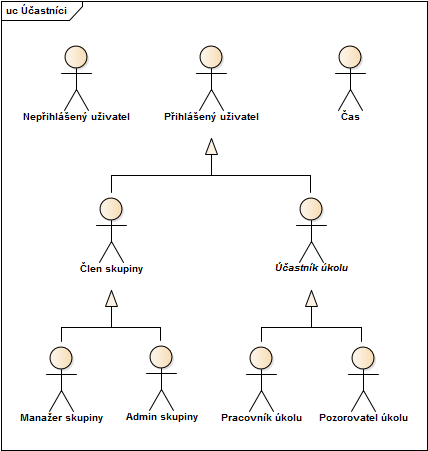
\includegraphics[width=0.7\textwidth]{ea-diagrams/uc-actors.png}
				\caption[Diagram účastníků]{Diagram účastníků aplikace}
				\label{diagram:actors}
			\end{figure}
			
			
			
		\subsection{Případy užití}
			%TODO - scénáře užití aby začínaly "Scénář začíná, když ..."
			Případy užití získané analýzou \textit{user stories} zobrazuji v diagramech případů užití. Rozdělil jsem je do čtyř balíků podle jejich účastníků pro lepší přehlednost.
			
			\subsubsection{Nepřihlášený uživatel}
			V diagramu \ref{diagram:uc-unauthorized} jsou zachyceny případy užití pro Nepřihlášeného uživatele.
			\begin{figure}\centering
				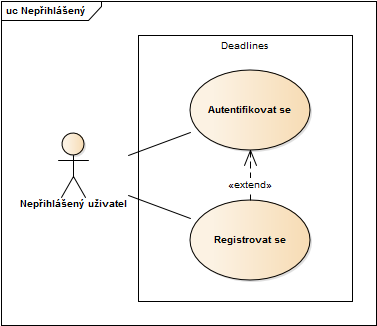
\includegraphics[width=0.7\textwidth]{ea-diagrams/uc-unauthorized.png}
				\caption[Případy užití nepřihlášených uživatelů]{Diagram případů užití pro nepřihlášeného uživatele}
				\label{diagram:uc-unauthorized}
			\end{figure}
			
			\begin{description}
				\item[UC 1.01 Registrovat se] \hfill \\
					Umožní uživateli aplikace zaregistrovat se. Zadá svůj e-mail, heslo a jméno.
					
				\item[UC 1.02 Přihlásit se] \hfill \\
					Umožní uživateli přihlásit se pomocí svého e-mailu a hesla.	
					
			\end{description}
		
		
		
		
		
		
			\subsubsection{Případy užití pro jednotlivce}	
			V diagramu \ref{diagram:uc-logged-user} a \ref{diagram:uc-task-members} jsou zachyceny případy užití aplikace jednotlivci. V prvním diagramu jsou případy užití z pohledu Přihlášeného uživatele v druhém pak z pohledu Pozorovatele a Pracovníka úkolu.
			
			
			
			\begin{description}
				\item[UC 2.01 Odhlásit se] \hfill \\
					Odhlásí uživatele z aplikace.
					
				\item[UC 2.02 Upravit svůj profil] \hfill \\
					Umožní uživateli upravit si své jméno a heslo.
				
				\item[UC 2.03 Vytvořit úkol] \hfill \\
					1. Uživatel chce vytvořit úkol \\
					2. Uživatel vyplní informace k úkolu, povinně název a typ. Pokud je typ \uv{S deadlinem},  pak je povinné i datum a čas deadlinu. Volitelně může zadat popis, pracnost v \textit{manhours} a prioritu jako celé číslo v intervalu 1--5. \\
					3. <Sdílet úkol> \\
					4. Aplikace vytvoří úkol, uživatel se stane jeho Pracovníkem. \\
				
				\item[UC 2.04 Sdílet úkol] \hfill \\
					1. Uživatel chce sdílet úkol. \\
					2. <Zobrazit seznam uživatelů> \\
					3. <Zobrazit seznam skupin> \\
					3. Uživatel určí uživatele a skupiny, se kterými chce úkol sdílet. \\
					4. Aplikace pošle vybraným uživatelům a skupinám nabídku ke sdílení úkolu.
				
				\item[UC 2.05 Zobrazit seznam mých úkolů] \hfill \\
				    1. <Filtrovat úkoly> \\
				    2. <Řadit úkoly> \\
					3. Aplikace zobrazí seznam všech úkolů, kterých je uživatel součástí, se zvoleným filtrem a řazením. Výchozí řazení je podle urgentnosti. \\
					
				\item[UC 2.06 Filtrovat úkoly] \hfill \\
					Úkoly je možné filtrovat podle role uživatele v nich (pozorovatel nebo pracovník), podle jejich typu (s deadlinem nebo rostoucí), stavu (otevřený, splněný nebo zavřený) a priority (celé číslo 1--5).
					
				\item[UC 2.07 Řadit úkoly] \hfill \\
					Úkoly je možné řadit podle zvoleného kritéria. Tím může být název, datum začátku nebo \textit{deadlinu} úkolu, rozpracovanost (v procentech odpracováno ku celkové pracnosti), priorita a urgentnost.
				
				\item[UC 2.08 Rozhodnout o příchozí nabídce sdílení úkolu] \hfill \\
					1. <Zobrazit seznam příchozích nabídek na sdílení úkolu> \\
					2. Uživatel rozhodne, zda chce nabídku přijmout, nebo zamítnout. \\
					3. Pokud je nabídka přijata, stává se uživatel pozorovatelem sdíleného úkolu. V opačném případě je nabídka smazána. \\
				
				\item[UC 2.09 Zobrazit seznam nabídek na sdílení úkolu] \hfill \\
					Zobrazí seznam nabídek pro uživatele k připojení se ke sdílenému úkolu, v němž bude u každé nabídky uvedeno jméno sdílejícího uživatele a název úkolu.
				
				\item[UC 2.10 Založit pracovní skupinu] \hfill \\
					1. Uživatel chce založit pracovní skupinu \\
					2. <Zobrazit seznam uživatelů> \\
					3. Uživatel zadá jméno skupiny a volitelně její popis. Dále zadá seznam e-mailů uživatelů, které chce do skupiny pozvat. \\
					4. Aplikace vytvoří novou skupinu s daným názvem a popisem. Zakládající uživatel se stane jejím Adminem. \\
					5. Aplikace rozešle nabídky ke vstupu do skupiny zadaným uživatelům. \\
					
				\item[UC 2.11 Rozhodnout o příchozí nabídce ke vstupu do skupiny] \hfill \\
					Uživatel rozhodne, zda chce přijmout nebo odmítnout nabídku ke vstupu do skupiny. Pokud ji přijme, stane se jejím Členem.
					
				\item[UC 2.12 Zobrazit seznam nabídek ke vstupu do skupiny] \hfill \\
					Zobrazí seznam nabídek ke vstupu do skupin. U každé nabídky bude uvedeno jméno skupiny a jméno a e-mail uživatele, od něhož nabídka pochází.
				
				\item[UC 2.13 Zobrazit seznam uživatelů] \hfill \\
					Zobrazí seznam uživatelů aplikace. U uživatele bude uvedeno jeho jméno a e-mail.
					
				\item[UC 2.14 Zobrazit seznam skupin] \hfill \\
					Zobrazí seznam skupin v aplikaci. U skupiny bude uvedeno její jméno a admin.
					
				\item[UC 2.15 Zobrazit úkol] \hfill \\
					1. Uživatel chce zobrazit detaily úkolu \\
					2. <Zobrazit seznam mých úkolů> \\
					3. Aplikace zobrazí všechny informace o úkolu, tedy název, popis, datum a čas začátku a \textit{deadlinu}, pracnost, prioritu, typ, stav a seznam jeho Pracovníků a Pozorovatelů. \\
					
					
				%%%%%%%%%%%%%%%%%%%%%%%%%%%%%%%%%%%%%%%%%%%%%%%%%%%%%%%%%%%%%%%
				% Diagramy %
				%%%%%%%%%%%%
				\begin{figure}\centering
					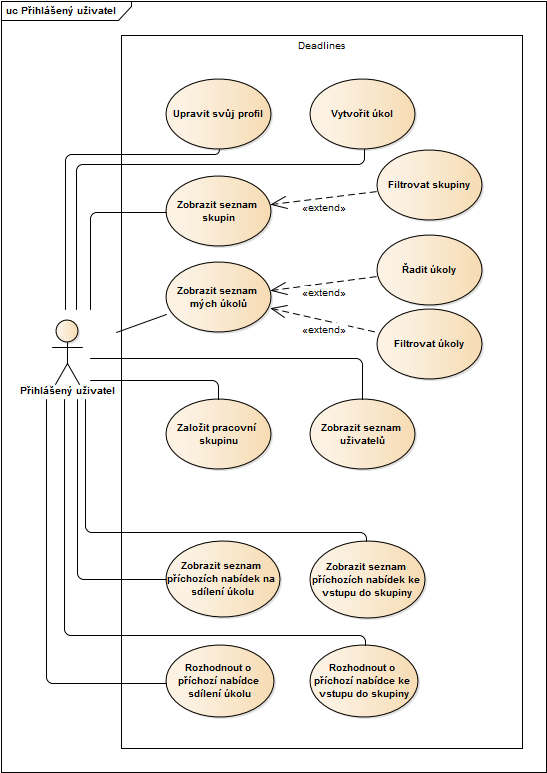
\includegraphics[width=0.9\textwidth]{ea-diagrams/uc-logged-user.png}
					\caption[Případy užití přihlášeného uživatele]{Diagram případů užití pro přihlášeného uživatele}
					\label{diagram:uc-logged-user}
				\end{figure}
				
				\begin{figure}\centering
					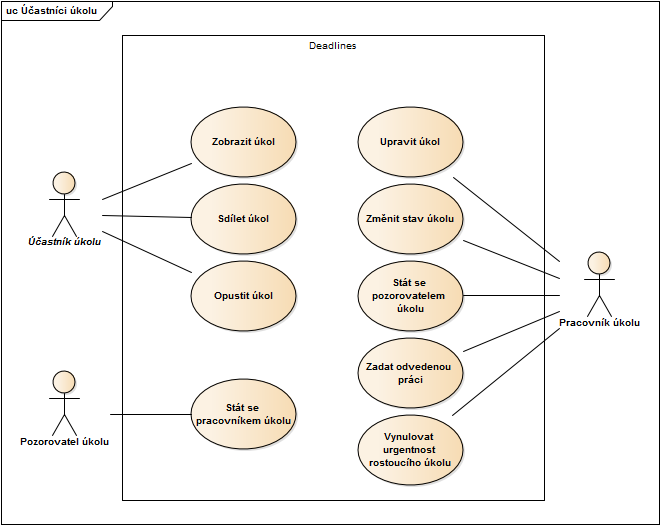
\includegraphics[width=0.7\textwidth]{ea-diagrams/uc-task-members.png}
					\caption[Případy užití účastníky úkolu]{Diagram případů užití pro účastníky úkolu}
					\label{diagram:uc-task-members}
				\end{figure}
				%%%%%%%%%%%%%%%%%%%%%%%%%%%%%%%%%%%%%%%%%%%%%%%%%%%%%%%%%%%%%%%
				
				
				\item[UC 2.16 Stát se pracovníkem úkolu] \hfill \\
					Umožňuje Pozorovateli úkolu stát se jeho Pracovníkem.				
								
				\item[UC 2.17 Změnit stav úkolu] \hfill \\
					Umožňuje Pracovníkovi změnit stav úkolu na jakýkoliv z jeho možných stavů.
				
				\item[UC 2.18 Upravit úkol] \hfill \\
					Umožňuje Pracovníkovi upravit u úkolu jeho popis, \textit{deadline}, pracnost a prioritu.
				
				\item[UC 2.19 Stát se pozorovatelem úkolu] \hfill \\
					Umožňuje Pracovníkovi úkolu stát se jeho Pozorovatelem.
					
				\item[UC 2.20 Zadat odvedenou práci] \hfill \\
					Umožňuje Pracovníkovi zadat u úkolu odvedenou práci.
					
					%TODO - chci umožnit měření času?
					\begin{description}
						\item[Hlavní scénář]: Pracovník chce zadat počet odpracovaných hodin. \\
						1. Include(Zobrazit úkol) \\
						2. Uživatel zadá počet odpracovaných hodin a potvrdí. \\
						3. Aplikace k úkolu přidá zadaný počet hodin. \\
						
						\item[Alternativní scénář]: Pracovník chce měřit odpracovaný čas.
						1. Include(Zobrazit úkol)
						2. 
					\end{description}
					
					
					
				\item[UC 2.21 Vynulovat urgentnost rostoucího úkolu] \hfill \\
					Umožňuje Pracovníkovi vynulovat urgentnost rostoucího úkolu.
					
				\item[UC 2.21 Opustit úkol] \hfill \\
					Umožňuje Účastníkovi úkolu opustit ho. Účastníkem úkolu je možné být přímo a/nebo skrze skupinu. Opustit úkol lze pouze, pokud je Účastník součástí úkolu přímo.
				
					1. Případ užití začíná, když se Účastník úkolu rozhodne opustit úkol. \\
					2. Include(Zobrazit úkol) \\
					3. Účastník zašle požadavek na opuštění úkolu. \\
					4. Pokud nebyl úkol sdílen přímo s Účastníkem (ale skupinou, ve které je Členem), scénář končí. \\
					5. Aplikace odebere Účastníka z úkolu. Pokud byl ale Účastník navíc součástí úkolu skrze skupinu, jíž je členem, nadále zůstane součástí úkolu skrze tuto skupinu.
			\end{description}
			
			
			
			
			
			
			
			
			\subsubsection{Případy užití pro skupiny}
			V diagramu \ref{diagram:uc-shared} jsou zachyceny případy užití aplikace členy pracovních skupin. Týkají se správy skupinových úkolů a skupin samotných. 
			
			% TODO Pokud je diagram moc velký, přesunout do přílohy?
			\begin{figure}\centering
				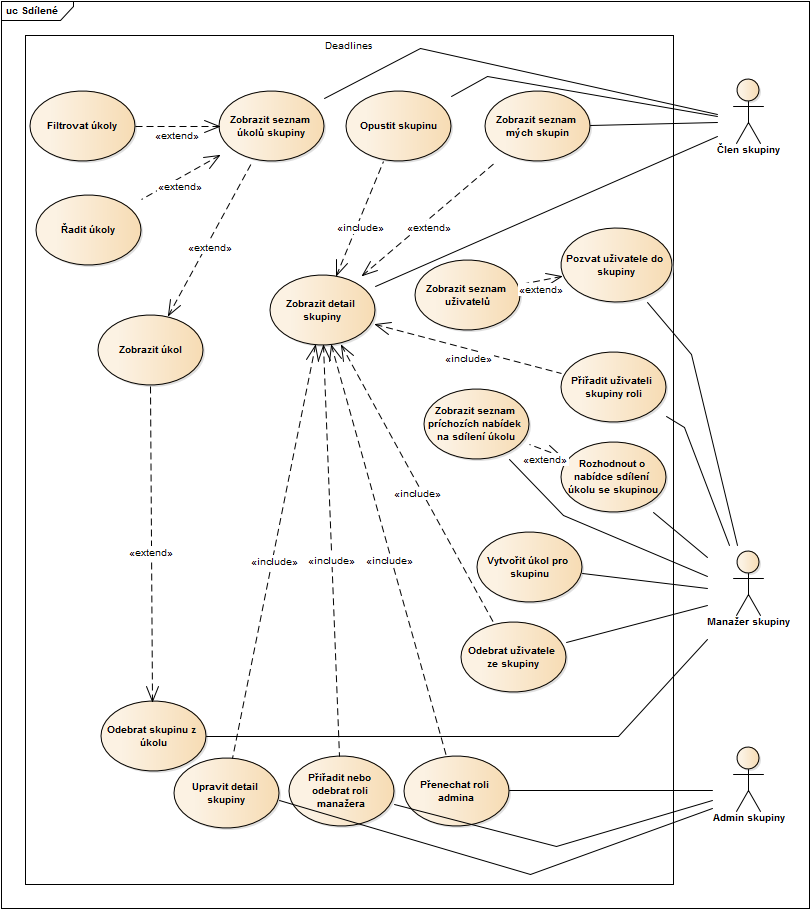
\includegraphics[width=1.0\textwidth]{ea-diagrams/uc-shared.png}
				\caption[Případy užití skupin]{Diagram případů užití pro členy pracovní skupiny}
				\label{diagram:uc-shared}
			\end{figure}
			
			\begin{description}
				\item[UC 3.01 Zobrazit seznam úkolů skupiny] \hfill \\
					1. Člen skupiny chce zobrazit úkoly své skupiny \\
					2. <Filtrovat úkoly> \\
					3. <Řadit úkoly> \\
					4. Aplikace zobrazí seznam všech úkolů skupiny se zvoleným filtrem a řazením. Výchozí řazení je podle urgentnosti. \\
					
				\item[UC 3.02 Opustit skupinu] \hfill \\
					1. Člen chce opustit skupinu. \\
					2. Include(Zobrazit detail skupiny) \\
					3. Člen zašle požadavek na opuštění skupiny. \\
					4. Pokud je Člen Adminem skupiny, opuštění je zamítnuto a scénář končí. \\
					5. Aplikace odebere Člena ze skupiny a ze všech úkolů, jichž byl součástí skrze opouštěnou skupinu.
				
				\item[UC 3.03 Zobrazit seznam mých skupin] \hfill \\
					Zobrazí Členovi seznam názvů všech skupin, ve kterých je Členem.
				
				\item[UC 3.04 Zobrazit detail skupiny] \hfill \\
					1. <Zobrazit seznam mých skupin> \\
					2. Člen zvolí skupinu, u které chce zobrazit detaily, a pošle požadavek. \\
					3. Pokud Člen nepatří do zvolené skupiny, je zobrazení odepřeno a scénář končí. \\
					4. Aplikace zobrazí detaily skupiny, tedy její jméno, popis, seznam Členů, Manažerů a Admina.
				
				\item[UC 3.05 Pozvat uživatele do skupiny] \hfill \\
					1. Případ užití začíná, když Manažer chce pozvat uživatele do skupiny. \\
					2. <Zobrazit seznam uživatelů> \\
					3. Manažer vybere uživatele, kterého chce pozvat, a pošle požadavek. \\
					4. Aplikace zašle uživateli nabídku ke vstupu do skupiny. \\
				
				\item[UC 3.06 Přiřadit Členovi roli na úkolu] \hfill \\
					Umožňuje přiřadit Členům skupiny roli Pozorovatele nebo Pracovníka na úkolech skupiny.
					
				\item[UC 3.07 Zobrazit seznam nabídek na sdílení úkolu se skupinou] \hfill \\
					Zobrazí seznam příchozích nabídek ke sdílení úkolů. U nabídky bude jméno uživatele, od kterého pochází, a název úkolu, kterého se týká.
					
				\item[UC 3.08 Rozhodnout o nabídce sdílení úkolu se skupinou] \hfill \\
					1. Případ užití začíná, když Manažer chce rozhodnout o nabídce sdílení úkolu se skupinou. \\
					2. <Zobrazit seznam nabídek na sdílení úkolu se skupinou> \\
					3. Pokud Manažer nabídku odmítne, je smazána a scénář končí. \\
					4. Pokud Manažer nabídku přijme, Aplikace úkol zařadí mezi úkoly skupiny a všichni Členové skupiny se stanou jeho Pozorovateli.
				
				\item[UC 3.09 Vytvořit úkol pro skupinu] \hfill \\
					1. Případ užití začíná, když Manažer chce vytvořit úkol pro skupinu. \\
					2. Manažer vyplní informace k úkolu, povinně název a typ. Pokud je typ \uv{S deadlinem}, pak je povinné i datum a čas deadlinu. Volitelně může zadat popis, pracnost v \textit{manhours} a prioritu jako celé číslo v intervalu 1--5. Zadá také skupinu, pro kterou chce úkol vytvořit. \\
					3. Pokud Manažer není Manažerem zvolené skupiny, vytvoření úkolu selže a scénář končí. \\
					4. Aplikace vytvoří úkol se zadanými parametry a přidá ho do úkolů skupiny, s níž byl sdílen. \\
					5. Aplikace přiřadí na úkolu všem Členům skupiny roli Pozorovatel.
				
				\item[UC 3.10 Odebrat uživatele ze skupiny] \hfill \\
					Umožňuje Manažerovi odebrat zvoleného uživatele ze skupiny. Ten je odebrán ze všech úkolů, jichž byl součástí skrze skupinu. Pokud se jedná o Manažera nebo Admina, je odebrání zakázáno. 
				
				\item[UC 3.11 Odebrat skupinu z úkolu] \hfill \\
					1. Případ užití začíná, když chce Manažer odebrat skupinu z úkolu, aby už nebyla jeho součástí. \\
					2. <Zobrazit úkol> \\
					3. <Zobrazit seznam úkolů skupiny> \\
					4. Manažer vybere úkol, ze kterého chce skupinu odebrat, a zašle požadavek. \\
					5. Aplikace u úkolu odebere sdílení se skupinou a odebere z úkolu všechny Členy skupiny, pokud nejsou součástí úkolu i mimo skupinu. \\
					
				\item[UC 3.12 Upravit detail skupiny] \hfill \\
					Umožňuje Adminovi měnit popis skupiny.
				
				\item[UC 3.13 Přiřadit nebo odebrat roli manažera] \hfill \\
					Umožňuje Adminovi přiřazovat a odebírat roli Manažera u všech Členů skupiny.
					
				\item[UC 3.14 Přenechat roli admina] \hfill \\
					Umožňuje Adminovi přenechat svou roli jinému členovi skupiny.
					
				\item[UC 3.15 Smazat skupinu] \hfill \\
					1. Případ užití začíná, když se Admin rozhodne smazat skupinu. \\
					2. Include(Zobrazit detail skupiny) \\
					3. Admin zašle požadavek na smazání skupiny. \\
					4. Pokud Admin není Adminem ve skupině, kterou chce smazat, scénář končí. \\
					5. Aplikace odebere všechny ostatní členy ze skupiny (\uv{Odebrat uživatele ze skupiny}). \\
					6. Aplikace odebere skupinu ze všech jejích úkolů (\uv{Odebrat skupinu z úkolu}). \\
					7. Aplikace odebere Admina ze skupiny. \\
					8. Aplikace smaže skupinu. \\
					
			\end{description}
				
				
			
			Diagram \ref{diagram:uc-time} zachycuje časově závislé případy užití, které se pravidelně vykonávají bez přičinění uživatelů aplikace.
			\begin{figure}\centering
				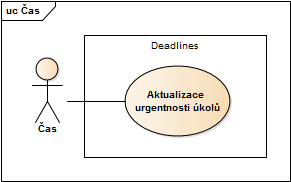
\includegraphics[width=0.5\textwidth]{ea-diagrams/uc-time.png}
				\caption[Případy užití časových událostí]{Diagram případů užití pro časově závislé události}
				\label{diagram:uc-time}
			\end{figure}
			
			\begin{description}
				\item[UC 4.01 Zvýšení urgentnosti rostoucích úkolů] \hfill \\
					1. Případ užití začíná po uplynutí časového intervalu pro zvyšování urgentnosti rostoucích úkolů. \\
					2. Aplikace u všech úkolů typu \uv{rostoucí} zvýší urgentnost o hodnotu danou nastavením úkolu. \\
				
				\item[UC 4.02 Aktualizace urgentnosti úkolů] \hfill \\
					1. Případ užití začíná po uplynutí časového intervalu pro aktualizaci urgentnosti úkolů. \\
					2. Aplikace u všech úkolů typu \uv{s deadlinem} vypočte novou hodnotu urgentnosti. \\
			\end{description}
			
			
			
			
			
		
		

		
	\section{Doménový model}
	% TODO podívat se na http://stackoverflow.com/questions/36100826/uml-domain-model-how-to-model-multiple-roles-of-association-between-two-entiti/36101591   -- možná upravit model?
		Doménový model slouží k popisu dat, zachycení hlavních entit, se kterými bude aplikace pracovat, a vztahů mezi nimi. \cite{domain-model} Jedná se o abstraktní pohled na problém, a tak diagram obsahuje jen entity a jejich vlastnosti dané předchozími kroky analýzy. Nejsou v něm implementační detaily, jako například konkrétní atributy a metody.
		
		Diagram doménového modelu je znázorněn na obrázku \ref{diagram:domain-model}. Znázorňuje vztahy mezi entitami a některá omezení, jako například vzájemnou výlučnost. \cite{domain-model-multiple-association} V této části se dále budu věnovat popisu jednotlivých entit modelu.
		
		\subsection{User}
			Entita User reprezentuje uživatele aplikace. Uchovává jeho e-mail, který je unikátní v rámci aplikace, jméno a heslo k jeho přihlášení.
			
		\subsection{Group}
			Entita Group reprezentuje pracovní skupinu. Má název a popis. Uživatelé s ní mohou být ve třech různých vztazích -- jako Člen, Manažer a Admin. Tyto vztahy jsou vzájemně vylučující, takže uživatel nemůže být zároveň například Člen a Manažer.
		
		\subsection{Task}
			Entita Task reprezentuje úkol. Obsahuje informace definované v předchozích krocích analýzy. Uživatel může být součástí úkolu jako pozorovatel, nebo pracovník. Nemůže být ale oboje zároveň. 
		
		\subsection{DeadlineTask}
			Entita DeadlineTask je typ entity Task, reprezentující úkol s \textit{deadlinem}. 
		
		\subsection{GrowingTask}
			Entita GrowingTask je typ entity Task, reprezentující rostoucí úkol. Obsahuje informaci o rychlosti růstu jeho urgentnosti.
		
		\subsection{TaskParticipant}
			TaskParticipant je entita reprezentující dvojici entit User--Group. Tato dvojice je v aplikaci unikátní, takže nemůžou existovat dvě stejné dvojice zároveň. 
			
			Skrze tuto entitu je uživatel součástí úkolu. Součástí úkolu může být sám, pokud není k entitě TaskParticipant přiřazena žádná skupina, nebo může být součástí úkolu jako člen skupiny, pokud k entitě skupina přiřazena je. Uživatel také může být součástí úkolu jako člen více skupin zároveň.
		
		\subsection{TaskWork}
			Entita TaskWork reprezentuje práci vykonanou na úkolu uživatelem. Je spjata s entitou User, místo TaskParticipant, takže i když uživatel úkol opustí, pořád bude záznam o jeho práci na úkolu existovat.
		
		\subsection{Offer}
			Entita Offer reprezentuje nabídku, kterou uživatel někomu zasílá.
		
		\subsection{TaskSharingOffer}
			Entita TaskSharingOffer je typ nabídky, která reprezentuje nabídku ke sdílení úkolu.
		
		\subsection{UserTaskSharingOffer}
			Entita UserTaskSharingOffer je typ nabídky ke sdílení úkolu, která je určena pro uživatele. Vznikne, pokud jeden uživatel chce k úkolu, na kterém pracuje, pozvat jiného uživatele.
		
		\subsection{GroupTaskSharingOffer}
			Entita UserTaskSharingOffer je typ nabídky ke sdílení úkolu, která je určena pro skupinu. Vznikne, pokud jeden uživatel chce k úkolu, na kterém pracuje, pozvat skupinu.
		
		\subsection{MembershipOffer}
			Entita MembershipOffer je typ nabídky, která reprezentuje nabídku ke vstupu do skupiny. Vznikne, pokud manažer skupiny do ní chce pozvat nového uživatele.
		
	
%%%%%%%%%%%%%%%%%%%%%%%%%%%%%%%%%%%%%%%%%%%%%%%%%%%%%%%%%%%%%%%%%%%%%%%%%%%%%%%%%%%%%%%%%%%%%%%%%%%%%%%%%
%%%%%%%%%%%%%%%%%%%%%%%%%%%%%%%%%%%%%%%%%%%%%%%%%%%%%%%%%%%%%%%%%%%%%%%%%%%%%%%%%%%%%%%%%%%%%%%%%%%%%%%%%

\chapter{Návrh řešení}
	\label{chapter:design}
	
	V této kapitole představím technologie zvolené k vypracování aplikace a navrhnu REST API, které bude aplikace nabízet. Dále se budu věnovat architektuře aplikace, návrhovému modelu tříd a databázovému modelu, což bude představovat podklad pro následující implementaci prototypu aplikace ve zvolené technologii.

	\section{Technologie}
	
		\subsection{Java}
			Již v zadání práce je avizováno, že aplikace bude postavena na platformě Java. \cite{java} Jazyk Java byl vyvinutý společností Sun Microsystems a veřejnosti představen v roce 1996. Syntaxí je podobný C/C++ a je silně objektově orientovaný. Program napsaný v Javě je kompilován do podoby \textit{bytecode}, který je následně spouštěn na \textit{Java Virtual Machine} (JVM), který bytecode interpretuje. To znamená, že jazyk je platformně nezávislý -- \textit{bytecode} vzniklý kompilací zdrojového Java kódu je možné spustit na jakékoliv platformě, pokud na ní je přítomný odpovídající \textit{JVM}. 
			
			Oproti jazykům C/C++ navíc Java disponuje automatickou správou paměti, nazvanou \textit{garbage collection}, takže vývojáři se nemusí tolik starat o životní cyklus objektů a následné \textit{memory leaks}. \cite{what-is-java} \cite{pjv-java}
		
		\subsection{Spring}
			Spring je framework, který zjednodušuje tvorbu enterprise aplikací v Javě. \cite{spring} Jednou z výhod Springu je jeho podpora návrhového vzoru \textit{dependency injection}, díky kterému je program lépe modularizovatelný, testovatelný a znovupoužitelný.\cite{dependency-injection}
			
			Další součástí Springu je webový modul \textit{Web MVC framework}. \cite{spring-mvc-framework} Ten umožňuje tvorbu webových aplikací podle architektonického vzoru MVC. Je také možné využít ho pro tvorbu \textit{RESTful} aplikace, což je cílem implementační části této práce.
			
			\subsubsection{Spring Boot}
				Nadstavbou k frameworku Spring je projekt Spring Boot. \cite{spring-boot} Vztah mezi Spring a Spring Boot je zobrazen na obrázku \ref{pic:spring-boot}. Byl vyvinut k usnadnění tvorby Spring aplikací. Představuje více \uv{dogmatický} (\textit{opinionated}) pohled na Spring, což znamená, že od vývojáře očekává \uv{standardní} chování podle zaběhlých postupů. \cite{opinionated-software} Vývojáře za to ale odstiňuje od nutnosti (nejen) počáteční konfigurace a nabízí navíc některé funkce, jako \textit{embedded server}, bezpečnost, metriky, kontrolu stavu aplikace a další. V případě, že výchozí konfigurace nevyhovuje, je možné si ji ručně přizpůsobit. \cite{spring-boot-blog}
				
				Spring Boot také umožňuje sestavit aplikaci do podoby jednoho JAR souboru (\uv{\textit{fat jar}}), který obsahuje vše, co je nutné k jejímu spuštění. Není tedy potřeba mít pro nasazení zprovozněný aplikační server, jako například Tomcat či GlassFish. Stále je ale možné aplikaci sestavit do WAR souboru a vlastní server použít.
				
				\begin{figure}\centering
					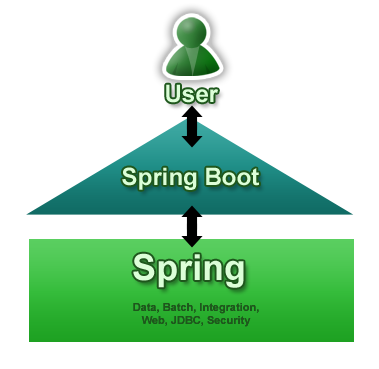
\includegraphics[width=0.5\textwidth]{spring-boot.png}
					\caption[Spring Boot]{Vztah Spring a Spring Boot \cite{spring-boot-blog}}
					\label{pic:spring-boot}
				\end{figure}
				
		\subsection{Hibernate}
			Hibernate \cite{hibernate} je framework pro platformu Java, usnadňující persistenci dat. Jedná se o nástroj pro ORM (objektově-relační mapování), který se stará o transformaci objektů aplikace do podoby vhodné pro uložení do relační databáze, jejich uložení, a následné načtení a transformaci z databáze zpět na objekty. Způsob mapování objektů do databáze lze nastavit buď v konfiguračním XML souboru, nebo přímo ve zdrojovém kódu anotacemi.
			
			Kromě usnadnění práce s databází je další výhodou Hibernate možnost jednoduché změny uložiště. Kód aplikace komunikuje s jeho API stejným způsobem, nehledě na typ databáze, ke které je připojen.
			
		\subsection{apiary/dredd?}
			% TODO - budu používate dredd na testování API?
		
		\subsection{MySQL}
			Persistence dat aplikace bude zprostředkována relační databází. Pro výběr databáze jsem se řídil jejich popularitou a podmínkou použití zdarma. Nejpopulárnější takovou databází je MySQL. \cite{db-ranking} Aplikace nebude mít takové požadavky na persistentní vrstvu, aby nějak ovlivnily výběr databáze. Funkce, které budou potřeba, splňují všechny uvažované možnosti. Větší popularita MySQL bude znamenat lepší podporu komunity a snažší řešení problémů během implementace.
			
		\subsection{Apache Tomcat}
			Pro nasazení aplikace bude použit server Apache Tomcat. \cite{tomcat} Je to \textit{lightweight} server, nenáročný na hardware a jednoduchý na zprovoznění. 
			
			V případě spuštění aplikace jako JAR souboru je v něm Tomcat automaticky zahrnutý.
	
	\section{REST API}
		V této sekci nejprve krátce vysvětlím pojmy API a REST API. Poté přistoupím ke konkrétnímu návrhu REST API pro aplikaci Deadlines.
	
		\subsection{API}
			API (\textit{Application Programming Interface}) slouží k jednoduché a spolehlivé komunikaci mezi aplikacemi nebo moduly aplikace. API představuje kontrakt, kterým se \textit{producent} zavazuje k nabízení svých služeb v dané zdokumentované podobě, jež mohou být využity \textit{konzumenty}.
			
			Autoři knihy \textit{APIs: A Strategy Guide} \cite{apis-a-strategy-guide} definují API takto:
			
			\textit{API je v podstatě kontrakt. Ve chvíli, kdy tento kontrakt existuje, vývojáři tíhnou k využívání API, protože ví, že se na něj mohou spolehnout. Kontrakt zvyšuje důvěru, což zlepšuje použitelnost. Tento kontrakt také zefektivňuje spojení mezi producentem a konzumentem, protože rozhraní jsou dokumentována, jsou konzistentní a předvídatelná.}
	
		\subsection{REST}
			Termín REST (REpresentational State Transfer) byl poprvé zaveden v roce 2000 Royem Fieldingem v jeho dizertační práci. \cite{rest-dissertation} Ve zkratce se jedná o koncept designu distribuované architektury. Definuje rozhraní, které je použitelné pro jednotný přístup ke zdrojům (resources). Těmi mohou být data nebo stavy aplikace, popsatelné konkrétními daty.
			Zdroje v kontextu REST jsou identifikované pomocí URI a komunikovány mezi klientem a serverem v podobě reprezentací v libovolné textové, strojově zpracovatelné podobě (například JSON nebo XML). \cite{rest-youtube}
			
			Architektonický styl REST popisuje šest podmínek:
			\begin{itemize}
				\item Uniform Interface (Jednotné rozhraní)
				\item Stateless (Bezstavovost)
				\item Cacheable (Cachovatelnost)
				\item Client-Server
				\item Layered System (Systém z vrstev)
				\item Code on Demand (Kód na vyžádání)
			\end{itemize}
			Popis architektury REST není předmětem této práce, takže se mu dále nebudu věnovat.
			
		\subsection{REST API aplikace Deadlines}
			API aplikace budu dokumentovat ve formátu API Blueprint. \cite{api-blueprint} Ten představuje jednoduchý způsob, jak popsat zdroje, jejich \textit{endpointy}, návratové hodnoty a další informace. Jeho syntaxe vychází z jazyka Markdown. \cite{markdown}
			
	
	\section{Architektura aplikace}
	\section{Návrhový model}
	\section{Databázový model}

%%%%%%%%%%%%%%%%%%%%%%%%%%%%%%%%%%%%%%%%%%%%%%%%%%%%%%%%%%%%%%%%%%%%%%%%%%%%%%%%%%%%%%%%%%%%%%%%%%%%%%%%%
%%%%%%%%%%%%%%%%%%%%%%%%%%%%%%%%%%%%%%%%%%%%%%%%%%%%%%%%%%%%%%%%%%%%%%%%%%%%%%%%%%%%%%%%%%%%%%%%%%%%%%%%%

\chapter{Implementace}
	\label{chapter:implementation}

%%%%%%%%%%%%%%%%%%%%%%%%%%%%%%%%%%%%%%%%%%%%%%%%%%%%%%%%%%%%%%%%%%%%%%%%%%%%%%%%%%%%%%%%%%%%%%%%%%%%%%%%%
%%%%%%%%%%%%%%%%%%%%%%%%%%%%%%%%%%%%%%%%%%%%%%%%%%%%%%%%%%%%%%%%%%%%%%%%%%%%%%%%%%%%%%%%%%%%%%%%%%%%%%%%%

\chapter{Testování}
	\label{chapter:testing}

%%%%%%%%%%%%%%%%%%%%%%%%%%%%%%%%%%%%%%%%%%%%%%%%%%%%%%%%%%%%%%%%%%%%%%%%%%%%%%%%%%%%%%%%%%%%%%%%%%%%%%%%%
%%%%%%%%%%%%%%%%%%%%%%%%%%%%%%%%%%%%%%%%%%%%%%%%%%%%%%%%%%%%%%%%%%%%%%%%%%%%%%%%%%%%%%%%%%%%%%%%%%%%%%%%%

\chapter{Nasazení}
	\label{chapter:deployment}

%%%%%%%%%%%%%%%%%%%%%%%%%%%%%%%%%%%%%%%%%%%%%%%%%%%%%%%%%%%%%%%%%%%%%%%%%%%%%%%%%%%%%%%%%%%%%%%%%%%%%%%%%
%%%%%%%%%%%%%%%%%%%%%%%%%%%%%%%%%%%%%%%%%%%%%%%%%%%%%%%%%%%%%%%%%%%%%%%%%%%%%%%%%%%%%%%%%%%%%%%%%%%%%%%%%

\begin{conclusion}
	TODO závěr
\end{conclusion}

\bibliographystyle{csn690}
\bibliography{melka-bibliography}

\appendix

\chapter{Seznam použitých zkratek}
% \printglossaries
\begin{description}
	\item[HW] Hardware
	\item[SW] Software
	\item[MVC] Model-View-Controller
\end{description}

\chapter{Splnění kritérií rešerše}
	\begin{center}
	\begin{threeparttable}
		\caption{Tabulka splnění kritérií rešerše}
		\label{table:criteria}
		\begin{tabular}{|c||c|c|c|c|c|c|}
			\hline
			           & Kr. 1 & Kr. 2 & Kr. 3 & Kr. 4 & Kr. 5 & Kr. 6 \\ \hline
			JIRA       & +     & ~     & ~     & ~     & +     & ~     \\ \hline
			Bugzilla   & +     & ~     & ~     & *     & +     & +     \\ \hline
			Redmine    & +     & ~     & ~     & *     & +     & +     \\ \hline
			Trello     & +     & +     & +     & +     & +     & ~     \\ \hline
			Trackie    & +     & +     & +     & ~     & ~     & ~     \\ \hline
			FogBugz    & +     & +     & ~     & ~     & +     & ~     \\ \hline
			Todoist    & +     & +     & +     & +     & +     & ~     \\ \hline
			Toodledo   & +     & ~     & +     & **    & +     & ~     \\ \hline
			Inbox      & +     & +     & ~     & +     & ~     & ~     \\ \hline
			Poznámky   & +     & +     & +     & +     & N/A   & N/A   \\ \hline
			
		\end{tabular}
		
		\begin{tablenotes}
			\item[+] Splněno
			\item[*] Zdarma na vlastním HW.
			\item[**] Zdarma jen bez spolupráce na úkolech
			\item Kr. 1 -- \crita
			\item Kr. 2 -- \critb
			\item Kr. 3 -- \critc
			\item Kr. 4 -- \critd
			\item Kr. 5 -- \critf
			\item Kr. 6 -- \critg
		\end{tablenotes}
		
	\end{threeparttable}
	\end{center}

\chapter{Doménový model}
		\begin{figure}\centering
			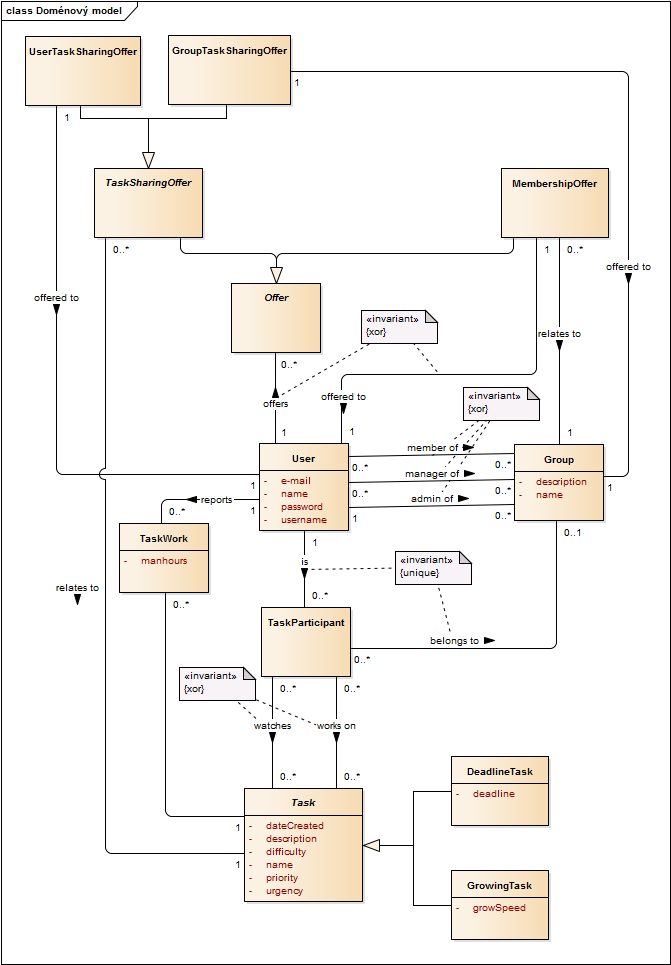
\includegraphics[width=1\textwidth]{ea-diagrams/domain-model.png}
			\caption[Doménový model]{Doménový model aplikace Deadlines}
			\label{diagram:domain-model}
		\end{figure}

\chapter{Obsah přiloženého CD}

%upravte podle skutecnosti

\begin{figure}
	\dirtree{%
		.1 readme.txt\DTcomment{stručný popis obsahu CD}.
		.1 exe\DTcomment{adresář se spustitelnou formou implementace}.
		.1 src.
		.2 impl\DTcomment{zdrojové kódy implementace}.
		.2 thesis\DTcomment{zdrojová forma práce ve formátu \LaTeX{}}.
		.1 text\DTcomment{text práce}.
		.2 thesis.pdf\DTcomment{text práce ve formátu PDF}.
		.2 thesis.ps\DTcomment{text práce ve formátu PS}.
	}
\end{figure}

\end{document}

% % % % % % % % % % % % % % % % % % % % % % % % % % % % 
% % Tuto kapitolu z výsledné práce ODSTRAŇTE.
% % % % % % % % % % % % % % % % % % % % % % % % % % % % 
% 
% \chapter{Návod k~použití této šablony}
% 
% Tento dokument slouží jako základ pro napsání závěrečné práce na Fakultě informačních technologií ČVUT v~Praze.
% 
% \section{Výběr základu}
% 
% Vyberte si šablonu podle druhu práce (bakalářská, diplomová), jazyka (čeština, angličtina) a kódování (ASCII, \mbox{UTF-8}, \mbox{ISO-8859-2} neboli latin2 a nebo \mbox{Windows-1250}). 
% 
% V~české variantě naleznete šablony v~souborech pojmenovaných ve formátu práce\_kódování.tex. Typ může být:
% \begin{description}
% 	\item[BP] bakalářská práce,
% 	\item[DP] diplomová (magisterská) práce.
% \end{description}
% Kódování, ve kterém chcete psát, může být:
% \begin{description}
% 	\item[UTF-8] kódování Unicode,
% 	\item[ISO-8859-2] latin2,
% 	\item[Windows-1250] znaková sada 1250 Windows.
% \end{description}
% V~případě nejistoty ohledně kódování doporučujeme následující postup:
% \begin{enumerate}
% 	\item Otevřete šablony pro kódování UTF-8 v~editoru prostého textu, který chcete pro psaní práce použít -- pokud můžete texty s~diakritikou normálně přečíst, použijte tuto šablonu.
% 	\item V~opačném případě postupujte dále podle toho, jaký operační systém používáte:
% 	\begin{itemize}
% 		\item v~případě Windows použijte šablonu pro kódování \mbox{Windows-1250},
% 		\item jinak zkuste použít šablonu pro kódování \mbox{ISO-8859-2}.
% 	\end{itemize}
% \end{enumerate}
% 
% 
% V~anglické variantě jsou šablony pojmenované podle typu práce, možnosti jsou:
% \begin{description}
% 	\item[bachelors] bakalářská práce,
% 	\item[masters] diplomová (magisterská) práce.
% \end{description}
% 
% \section{Použití šablony}
% 
% Šablona je určena pro zpracování systémem \LaTeXe{}. Text je možné psát v~textovém editoru jako prostý text, lze však také využít specializovaný editor pro \LaTeX{}, např. Kile.
% 
% Pro získání tisknutelného výstupu z~takto vytvořeného souboru použijte příkaz \verb|pdflatex|, kterému předáte cestu k~souboru jako parametr. Vhodný editor pro \LaTeX{} toto udělá za Vás. \verb|pdfcslatex| ani \verb|cslatex| \emph{nebudou} s~těmito šablonami fungovat.
% 
% Více informací o~použití systému \LaTeX{} najdete např. v~\cite{wikilatex}.
% 
% \subsection{Typografie}
% 
% Při psaní dodržujte typografické konvence zvoleného jazyka. České \uv{uvozovky} zapisujte použitím příkazu \verb|\uv|, kterému v~parametru předáte text, jenž má být v~uvozovkách. Anglické otevírací uvozovky se v~\LaTeX{}u zadávají jako dva zpětné apostrofy, uzavírací uvozovky jako dva apostrofy. Často chybně uváděný symbol "{} (palce) nemá s~uvozovkami nic společného.
% 
% Dále je třeba zabránit zalomení řádky mezi některými slovy, v~češtině např. za jednopísmennými předložkami a spojkami (vyjma \uv{a}). To docílíte vložením pružné nezalomitelné mezery -- znakem \texttt{\textasciitilde}. V~tomto případě to není třeba dělat ručně, lze použít program \verb|vlna|.
% 
% Více o~typografii viz \cite{kobltypo}.
% 
% \subsection{Obrázky}
% 
% Pro umožnění vkládání obrázků je vhodné použít balíček \verb|graphicx|, samotné vložení se provede příkazem \verb|\includegraphics|. Takto je možné vkládat obrázky ve formátu PDF, PNG a JPEG jestliže používáte pdf\LaTeX{} nebo ve formátu EPS jestliže používáte \LaTeX{}. Doporučujeme preferovat vektorové obrázky před rastrovými (vyjma fotografií).
% 
% \subsubsection{Získání vhodného formátu}
% 
% Pro získání vektorových formátů PDF nebo EPS z~jiných lze použít některý z~vektorových grafických editorů. Pro převod rastrového obrázku na vektorový lze použít rasterizaci, kterou mnohé editory zvládají (např. Inkscape). Pro konverze lze použít též nástroje pro dávkové zpracování běžně dodávané s~\LaTeX{}em, např. \verb|epstopdf|.
% 
% \subsubsection{Plovoucí prostředí}
% 
% Příkazem \verb|\includegraphics| lze obrázky vkládat přímo, doporučujeme však použít plovoucí prostředí, konkrétně \verb|figure|. Například obrázek \ref{fig:float} byl vložen tímto způsobem. Vůbec přitom nevadí, když je obrázek umístěn jinde, než bylo původně zamýšleno -- je tomu tak hlavně kvůli dodržení typografických konvencí. Namísto vynucování konkrétní pozice obrázku doporučujeme používat odkazování z~textu (dvojice příkazů \verb|\label| a \verb|\ref|).
% 
% \begin{figure}\centering
% 	
\includegraphics[width=0.5\textwidth, angle=30]{cvut-logo-bw}
% 	\caption[Příklad obrázku]{Ukázkový obrázek v~plovoucím prostředí}\label{fig:float}
% \end{figure}
% 
% \subsubsection{Verze obrázků}
% 
% % Gnuplot BW i barevně
% Může se hodit mít více verzí stejného obrázku, např. pro barevný či černobílý tisk a nebo pro prezentaci. S~pomocí některých nástrojů na generování grafiky je to snadné.
% 
% Máte-li například graf vytvořený v programu Gnuplot, můžete jeho černobílou variantu (viz obr. \ref{fig:gnuplot-bw}) vytvořit parametrem \verb|monochrome dashed| příkazu \verb|set term|. Barevnou variantu (viz obr. \ref{fig:gnuplot-col}) vhodnou na prezentace lze vytvořit parametrem \verb|colour solid|.
% 
% \begin{figure}\centering
% 	\includegraphics{gnuplot-bw}
% 	\caption{Černobílá varianta obrázku generovaného programem Gnuplot}\label{fig:gnuplot-bw}
% \end{figure}
% 
% \begin{figure}\centering
% 	\includegraphics{gnuplot-col}
% 	\caption{Barevná varianta obrázku generovaného programem Gnuplot}\label{fig:gnuplot-col}
% \end{figure}
% 
% 
% \subsection{Tabulky}
% 
% Tabulky lze zadávat různě, např. v~prostředí \verb|tabular|, avšak pro jejich vkládání platí to samé, co pro obrázky -- použijte plovoucí prostředí, v~tomto případě \verb|table|. Například tabulka \ref{tab:matematika} byla vložena tímto způsobem.
% 
% \begin{table}\centering
% 	\caption[Příklad tabulky]{Zadávání matematiky}\label{tab:matematika}
% 	\begin{tabular}{|l|l|c|c|}\hline
% 		Typ		& Prostředí		& \LaTeX{}ovská zkratka	& \TeX{}ovská zkratka	\tabularnewline \hline \hline
% 		Text		& \verb|math|		& \verb|\(...\)|	& \verb|$...$|		\tabularnewline \hline
% 		Displayed	& \verb|displaymath|	& \verb|\[...\]|	& \verb|$$...$$|	\tabularnewline \hline
% 	\end{tabular}
% \end{table}
% 
% % % % % % % % % % % % % % % % % % % % % % % % % % % % 